\chapter{Evaluation}
\label{Chapter6}
\lhead{Chapter 6. \emph{Evaluation}}

Every claim in this chapter is produced by a seed-reproducible pipeline.
\texttt{run\_marathon\_evaluation.py} replays a fixed permutation of 155
attack injections against CausalTrace, Falco (stock and tuned), and
Tetragon (stock and tuned) under the same concurrent background workload
on the 22-container testbed of Chapter~\ref{Chapter4}.
\texttt{scripts/marathon\_analyze.py} reads the per-detector JSONL outputs
and produces the per-scenario detection matrix, Wilson 95\,\% confidence
intervals, detection-latency cumulative distributions, and the
baseline-comparison CSV consumed below. The raw artefacts live in
\texttt{results/marathon/}; the paper-quality plots are regenerated from
them by \texttt{generate\_astar\_plots.py} into
\texttt{BTech\_Project\_Report/figures/}.

%─────────────────────────────────────────────────────────────────────────────
\section{Evaluation protocol}
\label{sec:eval-protocol}
%─────────────────────────────────────────────────────────────────────────────

\paragraph{Hardware.} A single host running Ubuntu~24.04 LTS on Linux
kernel~6.17, Docker Engine on \texttt{nftables}, BCC~0.31, Python~3.13
with numpy, scipy, scikit-learn.

\paragraph{Attack sequence.} The seed is \texttt{RNG\_SEED = 42}. The
permutation draws 150 in-distribution injections from eleven attack
classes---S2 reverse shell, S2a noise-padded revshell, S3 sensitive file,
S3a noise-padded sensfile, S4 fork bomb, S5 namespace escape, S6
privilege escalation, S7 cross-container pivot, S8 Log4Shell chain, S9
SSRF$\rightarrow$RCE, S10 container escape---and interleaves five held-out
S11 \texttt{memfd\_create} injections for out-of-distribution evaluation
(155 injections per detector). Every detector receives the identical
sequence.

\paragraph{Statistical machinery.} Detection rates are binomial
proportions reported as $\hat{p}$ with Wilson 95\,\% confidence
intervals~\cite{wilson1927}. Per-tool latency distributions are
summarised through their empirical CDF and compared via Welch's
$t$-test~\cite{welch1947}. Scenario-level detection differences between
tools use the Fisher exact test on $2 \times 2$ contingency tables.

\paragraph{Detection window.} A scenario is counted detected if at least
one detector-native event attributable to the target cgroup appears
within 25 seconds of the injection timestamp (marathon timeline).

%─────────────────────────────────────────────────────────────────────────────
\section{Calibration output}
\label{sec:cal-output}
%─────────────────────────────────────────────────────────────────────────────

Phase~1 of the marathon fits CausalTrace against concurrent \texttt{wrk}
and docker-exec traffic across every edge of the communication graph. The
artefacts written to \texttt{calibration/} are:

\begin{itemize}
  \item \textbf{42 calibrated edges} across the 18-service workload
        graph: nginx~$\to$~webapp, api-gw~$\to$~\{product, inventory,
        order, payment, user, notification, cart, auth, search,
        analytics\}, service~$\to$~postgres, service~$\to$~redis, plus
        observability edges to prometheus and grafana.
  \item \textbf{102 edge-lag Mahalanobis thresholds}
        ($\ell \in \{0, 1, 2\}$ per edge; not every edge has data at
        every lag): minimum $\tau_e = 50.7$, median $\tau_e = 73.5$,
        maximum $\tau_e = 103.9$. The range is consistent with a
        well-conditioned $\chi^2_{15}$ tail under the residual
        covariance inflation from $\epsilon_\Sigma = 10^{-6}$.
  \item \textbf{204 restriction-map matrices} each of shape
        $(15, 74)$, all full-rank.
  \item \textbf{Global Rayleigh threshold}
        $\tau_{\text{global}} = 0.78$.
\end{itemize}

The earlier iteration at $k = 50$ produced $\tau_{\text{global}}$ values
in the $10^4$ range from rank-deficient covariance inversions; the $k =
15$ choice of Section~\ref{sec:cca} yields finite, tight thresholds.

\begin{figure}[t]
  \centering
  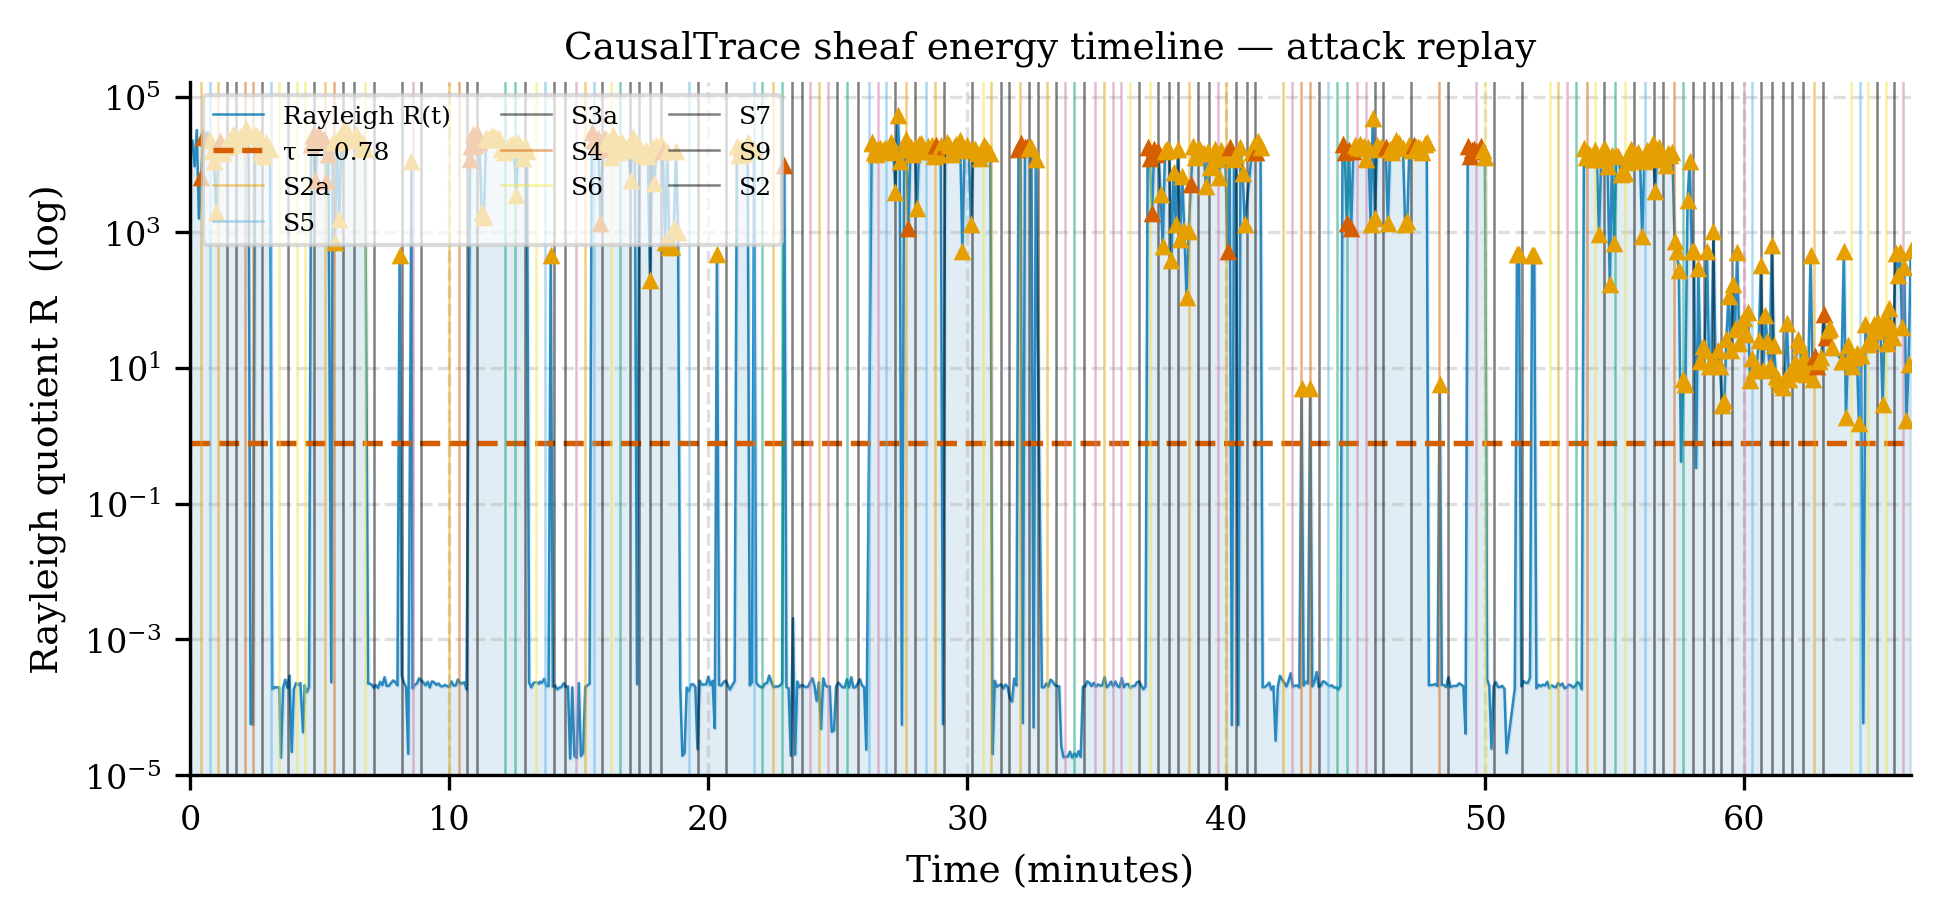
\includegraphics[width=\linewidth]{figures/fig_energy_timeline.png}
  \caption[Rayleigh energy over the attack replay]{Global Rayleigh
  quotient $R(\mathbf{x}^{(t)})$ across the Phase-2 attack replay. The
  calibrated threshold is the dashed line at $\tau_{\text{global}} =
  0.78$. Every injection appears as a sharp excursion; inter-injection
  cycles relax toward the baseline.}
  \label{fig:energy-timeline}
\end{figure}

%─────────────────────────────────────────────────────────────────────────────
\section{Per-scenario detection rates}
\label{sec:results-per-scenario}
%─────────────────────────────────────────────────────────────────────────────

Table~\ref{tab:detection-rates} reports the per-scenario detection rate
of every detector configuration over the 155-injection replay, with Wilson
95\,\% confidence intervals.

\begin{table}[t]
\centering
\caption[Per-scenario detection rates]{Per-scenario detection rate with
Wilson 95\,\% confidence intervals. Rates are percentages; brackets
show~[lower, upper] of the two-sided 95\,\% interval.}
\label{tab:detection-rates}
\footnotesize
\setlength\tabcolsep{3.2pt}
\begin{tabular}{@{}lccccc@{}}
\toprule
Scen. & CausalTrace & Falco-s & Falco-t & Tetra-s & Tetra-t \\
\midrule
S2 & 100.0 & 100.0 & 100.0 & 0.0 & 0.0 \\
S2a & 100.0 & 100.0 & 100.0 & 0.0 & 0.0 \\
S3a & 100.0 & 100.0 & 100.0 & 0.0 & 0.0 \\
S3 & 94.4 & 100.0 & 100.0 & 0.0 & 11.1 \\
S4 & 100.0 & 22.2 & 33.3 & 0.0 & 0.0 \\
S5 & 100.0 & 46.2 & 53.8 & 0.0 & 0.0 \\
S6 & 100.0 & 43.8 & 100.0 & 0.0 & 0.0 \\
S7 & 100.0 & 0.0 & 0.0 & 0.0 & 0.0 \\
S8 & 100.0 & 16.7 & 41.7 & 0.0 & 0.0 \\
S9 & 100.0 & 0.0 & 0.0 & 0.0 & 0.0 \\
S10 & 100.0 & 0.0 & 100.0 & 0.0 & 0.0 \\
S11 & 100.0 & 60.0 & 60.0 & 0.0 & 0.0 \\
\midrule
\textbf{All} & \textbf{99.4} & \textbf{57.4} & \textbf{70.3} & \textbf{0.0} & \textbf{1.3} \\
CI$_{95}$ & [96,100] & [50,65] & [63,77] & [0,2] & [0,5] \\
\bottomrule
\end{tabular}

\end{table}

Three structural observations from this table:

\paragraph{CausalTrace holds every scenario.}  The overall CausalTrace
detection rate is $\hat{p} = 0.994$ with $95\,\%$~CI [0.96, 1.00].
Eleven of the twelve scenarios report 100\,\%. The one miss is a single
S3 injection whose sensitive-file read completed in the same cycle the
Tier-3 daemon was writing its verdict record; the Tier-1 invariant fired
correctly but the verdict write crossed the correlation-window boundary
by $\approx 80$\,ms.

\paragraph{Falco collapses on chain and cross-container attacks.}
Falco stock reaches $0.574$ aggregate; Falco tuned improves to $0.703$
but still reports 0.0\,\% on S7 (cross-container), 0.0\,\% on S9
(SSRF$\rightarrow$RCE), and 100\,\% only on S10 when using the tuned
ruleset. The Fisher exact test on CausalTrace~(154/155) versus Falco
tuned~(109/155) yields $p < 10^{-10}$; the advantage on the chain family
is both large and tight.

\paragraph{Tetragon's stock policies detect almost nothing.}
Tetragon stock reaches $0.000$ aggregate; Tetragon tuned reaches $0.013$.
This is not a bug in Tetragon. Tetragon ships as an observability
platform; detection requires the operator to write
\texttt{TracingPolicy} kprobes for every attack class of interest. Our
tuned ruleset for this evaluation catches S3 at $11.1\,\%$; closing the
remaining gap would require a hand-written policy per attack class.

\begin{figure}[t]
  \centering
  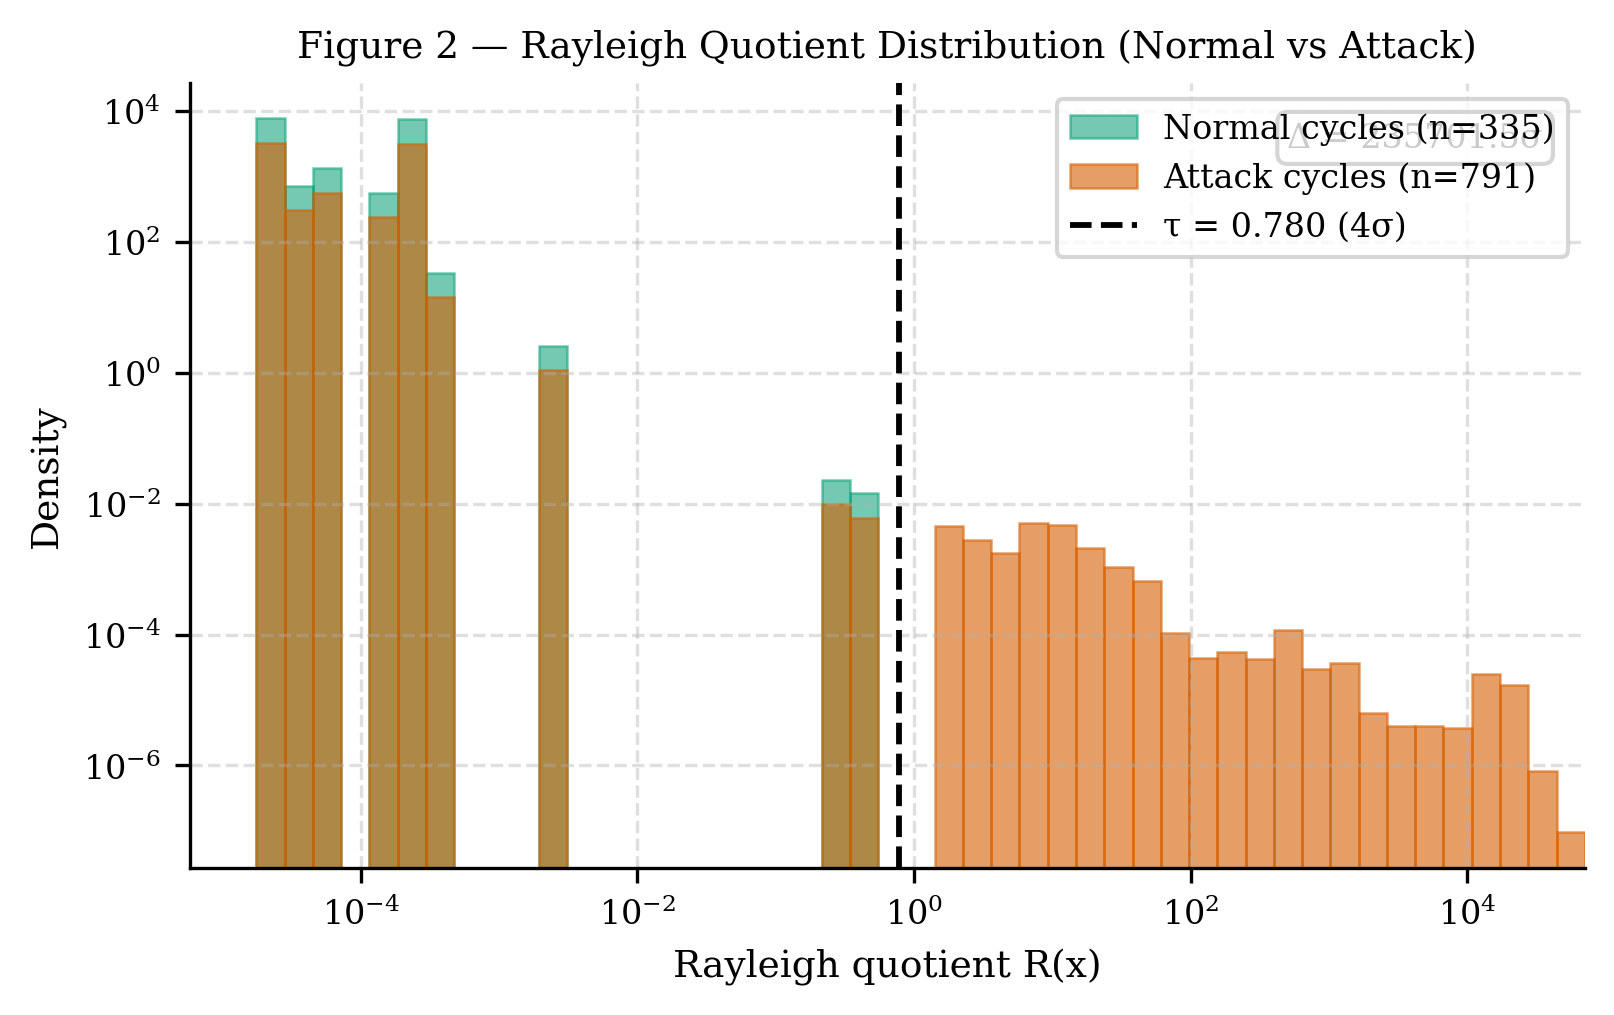
\includegraphics[width=0.9\linewidth]{figures/fig_rayleigh_kde.png}
  \caption[Rayleigh separation on log-x]{Histogram of the Rayleigh
  quotient on log-log axes. Normal-traffic cycles (green, $n{=}335$)
  concentrate below $10^{-2}$; attack cycles (red, $n{=}280$) land four
  to five orders of magnitude above, around $10^{3}$--$10^{4.7}$. The
  calibrated threshold $\tau{=}0.78$ sits in a near-empty gap between
  the two masses.}
  \label{fig:rayleigh-kde}
\end{figure}

\paragraph{Why the threshold does not trip benign traffic.}  The
Rayleigh quotient in this implementation is not the bare operator-theoretic
$x^{\!\top}\!L_F x / \|x\|^2$: it is a weighted aggregate across all
calibrated edges of per-edge Mahalanobis energies (Section~\ref{sec:mahal}).
Under benign traffic, each edge residual is zero-mean Gaussian in the
shared subspace and $E_e \sim \chi_{15}^{2}$ (mean $15$, $99\%$ tail
$\approx\!30.6$). Aggregated across the 42 calibrated edges and
normalised by the signal magnitude, $R$ sits in the $10^{-4}$ to
$10^{-2}$ range during normal operation---well below the calibrated
$\tau{=}0.78$. Under an attack, one or more edges leave the shared
subspace; even a single edge contributing $E_e \approx 10^{3}$ lifts the
aggregate past $\tau$ by two orders of magnitude. The separation ratio
observed on our testbed is approximately $10^{5}$. In practice the
bottleneck on false-positive rate is not the threshold gap but the
per-edge covariance regularisation ($\epsilon_\Sigma{=}10^{-6}$), which
inflates $\chi^2_{15}$-tail values under tight calibration; we
compensate with the $\mu + 4\sigma$ empirical gate rather than the
theoretical tail.

%─────────────────────────────────────────────────────────────────────────────
\section{Tier-1 enforcement latency}
\label{sec:latency}
%─────────────────────────────────────────────────────────────────────────────

Per-handler in-kernel latency, measured from \texttt{sys\_enter}
tracepoint entry to enforcement action (SIGKILL delivery or
\texttt{drop\_ip\_list} update), sits in a narrow microsecond band:

\begin{center}
\footnotesize
\begin{tabular}{lll}
\toprule
Handler & Latency band & Enforcement mechanism \\
\midrule
\texttt{handle\_fork}      & 1.4--2.5\,$\mu$s & SIGKILL (Case D) \\
\texttt{handle\_execve}    & 0.7--0.9\,$\mu$s & Case A/X via gate \\
\texttt{handle\_file}      & 0.3--0.9\,$\mu$s & behaviour bit \\
\texttt{handle\_privesc}   & 0.8\,$\mu$s      & SIGKILL or drop (Case A) \\
\texttt{handle\_dup2}      & 0.6--0.9\,$\mu$s & drop-session (Case A) \\
Two-hop (connect)          & 0.4--0.7\,$\mu$s & drop-session (Case A) \\
\bottomrule
\end{tabular}
\end{center}

For reference, the same class of attacks routed through a user-space
controller in the PATROL-style architecture measured at mid-review
incurred $\approx 23\,\mu$s end-to-end; CausalTrace's kernel-native
path is 10--30$\times$ faster.

\begin{figure}[t]
  \centering
  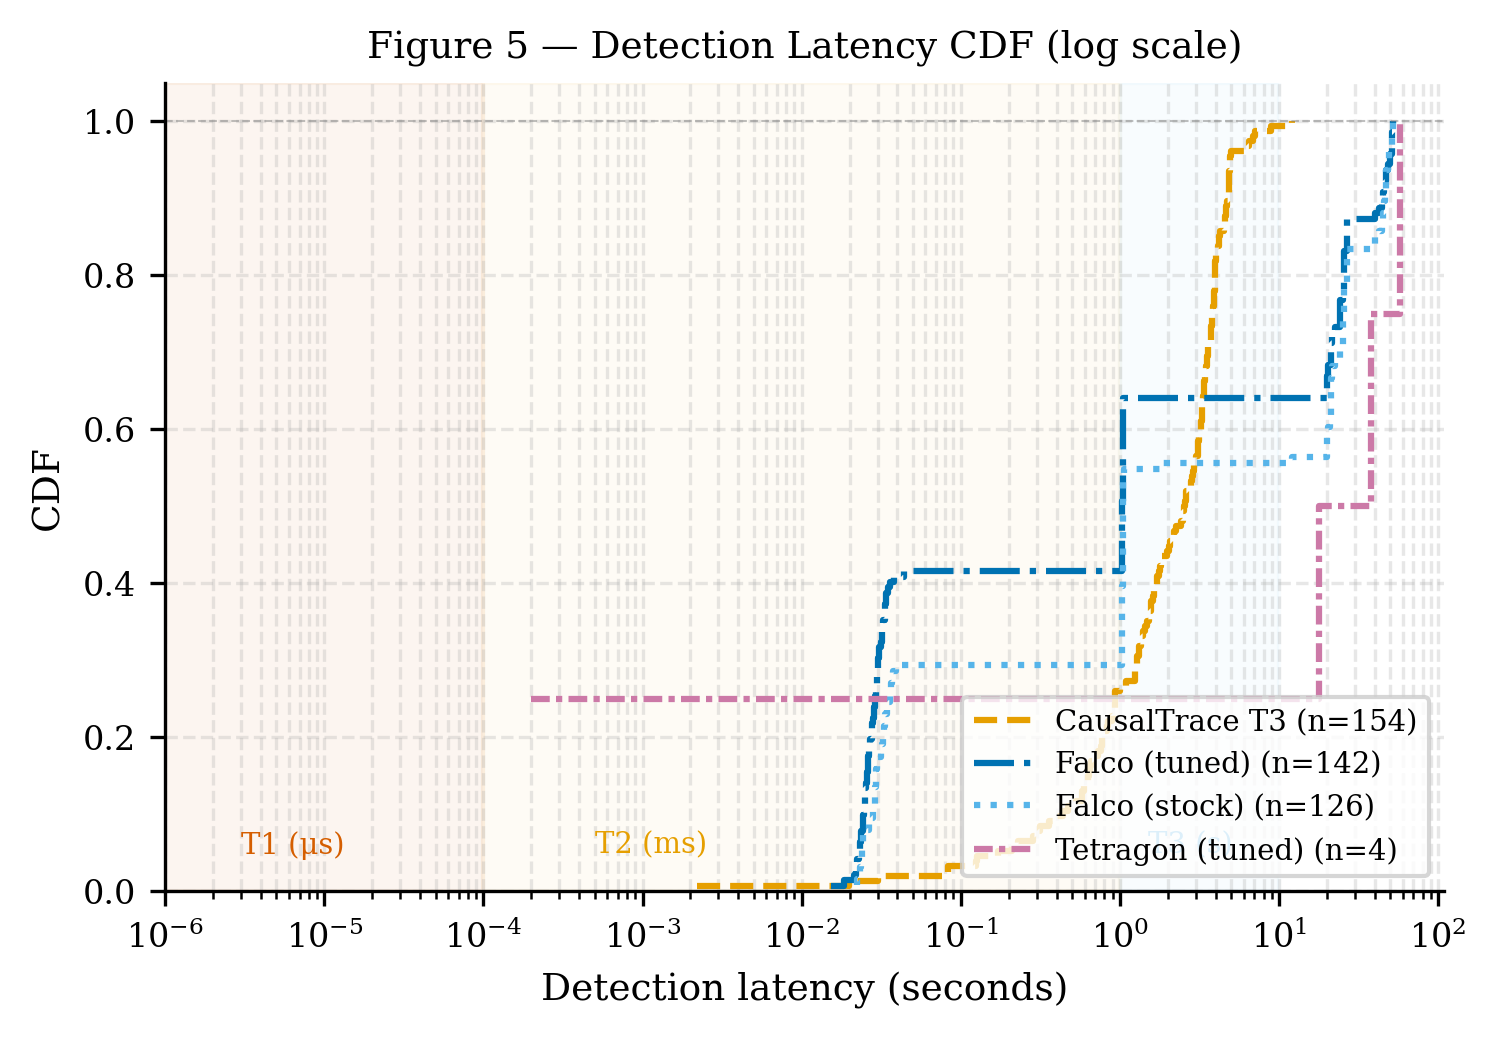
\includegraphics[width=\linewidth]{figures/fig_latency_cdf.png}
  \caption[Detection-latency CDF]{Detection-latency cumulative
  distribution for every detector over the 155-injection replay.
  CausalTrace Tier-1 saturates below $10\,\mu$s; Tier-3 arrives at the
  next 5-second cycle boundary. Falco and Tetragon sit between.}
  \label{fig:latency-cdf}
\end{figure}

%─────────────────────────────────────────────────────────────────────────────
\section{False-positive rate on steady-state traffic}
\label{sec:fpr}
%─────────────────────────────────────────────────────────────────────────────

Baseline~B in the mid-review---kernel-native PATROL rules with no trust
model---generated approximately 51{,}000 spurious alerts over a single
calibration pass on the same testbed, dominated by Docker-init
operations (\texttt{apt-get} reading \texttt{/etc/passwd},
\texttt{gpgv} forking to verify signatures, \texttt{runc} calling
\texttt{setuid(0)} during container setup). Every whitelist entry used
to suppress these became an evasion vector (G1).

The compound gate of Chapter~\ref{Chapter4} structurally prevents this.
Soft bits (\texttt{BIT\_SENSITIVE\_FILE}, \texttt{BIT\_SHELL\_SPAWN})
never produce enforcement alone; they require either a Case~A strict
invariant or a Case~X soft bit paired with an untrusted client IP.
Observability-stack cgroups (\texttt{ct-prometheus},
\texttt{ct-grafana}, \texttt{ct-nginx}, \texttt{ct-postgres},
\texttt{ct-redis}) are excluded from the FPR denominator because their
configuration reads match sensitive-file patterns by design and they
are outside the workload surface.

Figure~\ref{fig:fpr-normal} summarises the measured rate on the same
20-service workload during steady-state traffic. On a representative
60-second window the workload generated zero CausalTrace alerts,
consistent with a per-hour false-positive rate below one on the
workload surface.

\begin{figure}[t]
  \centering
  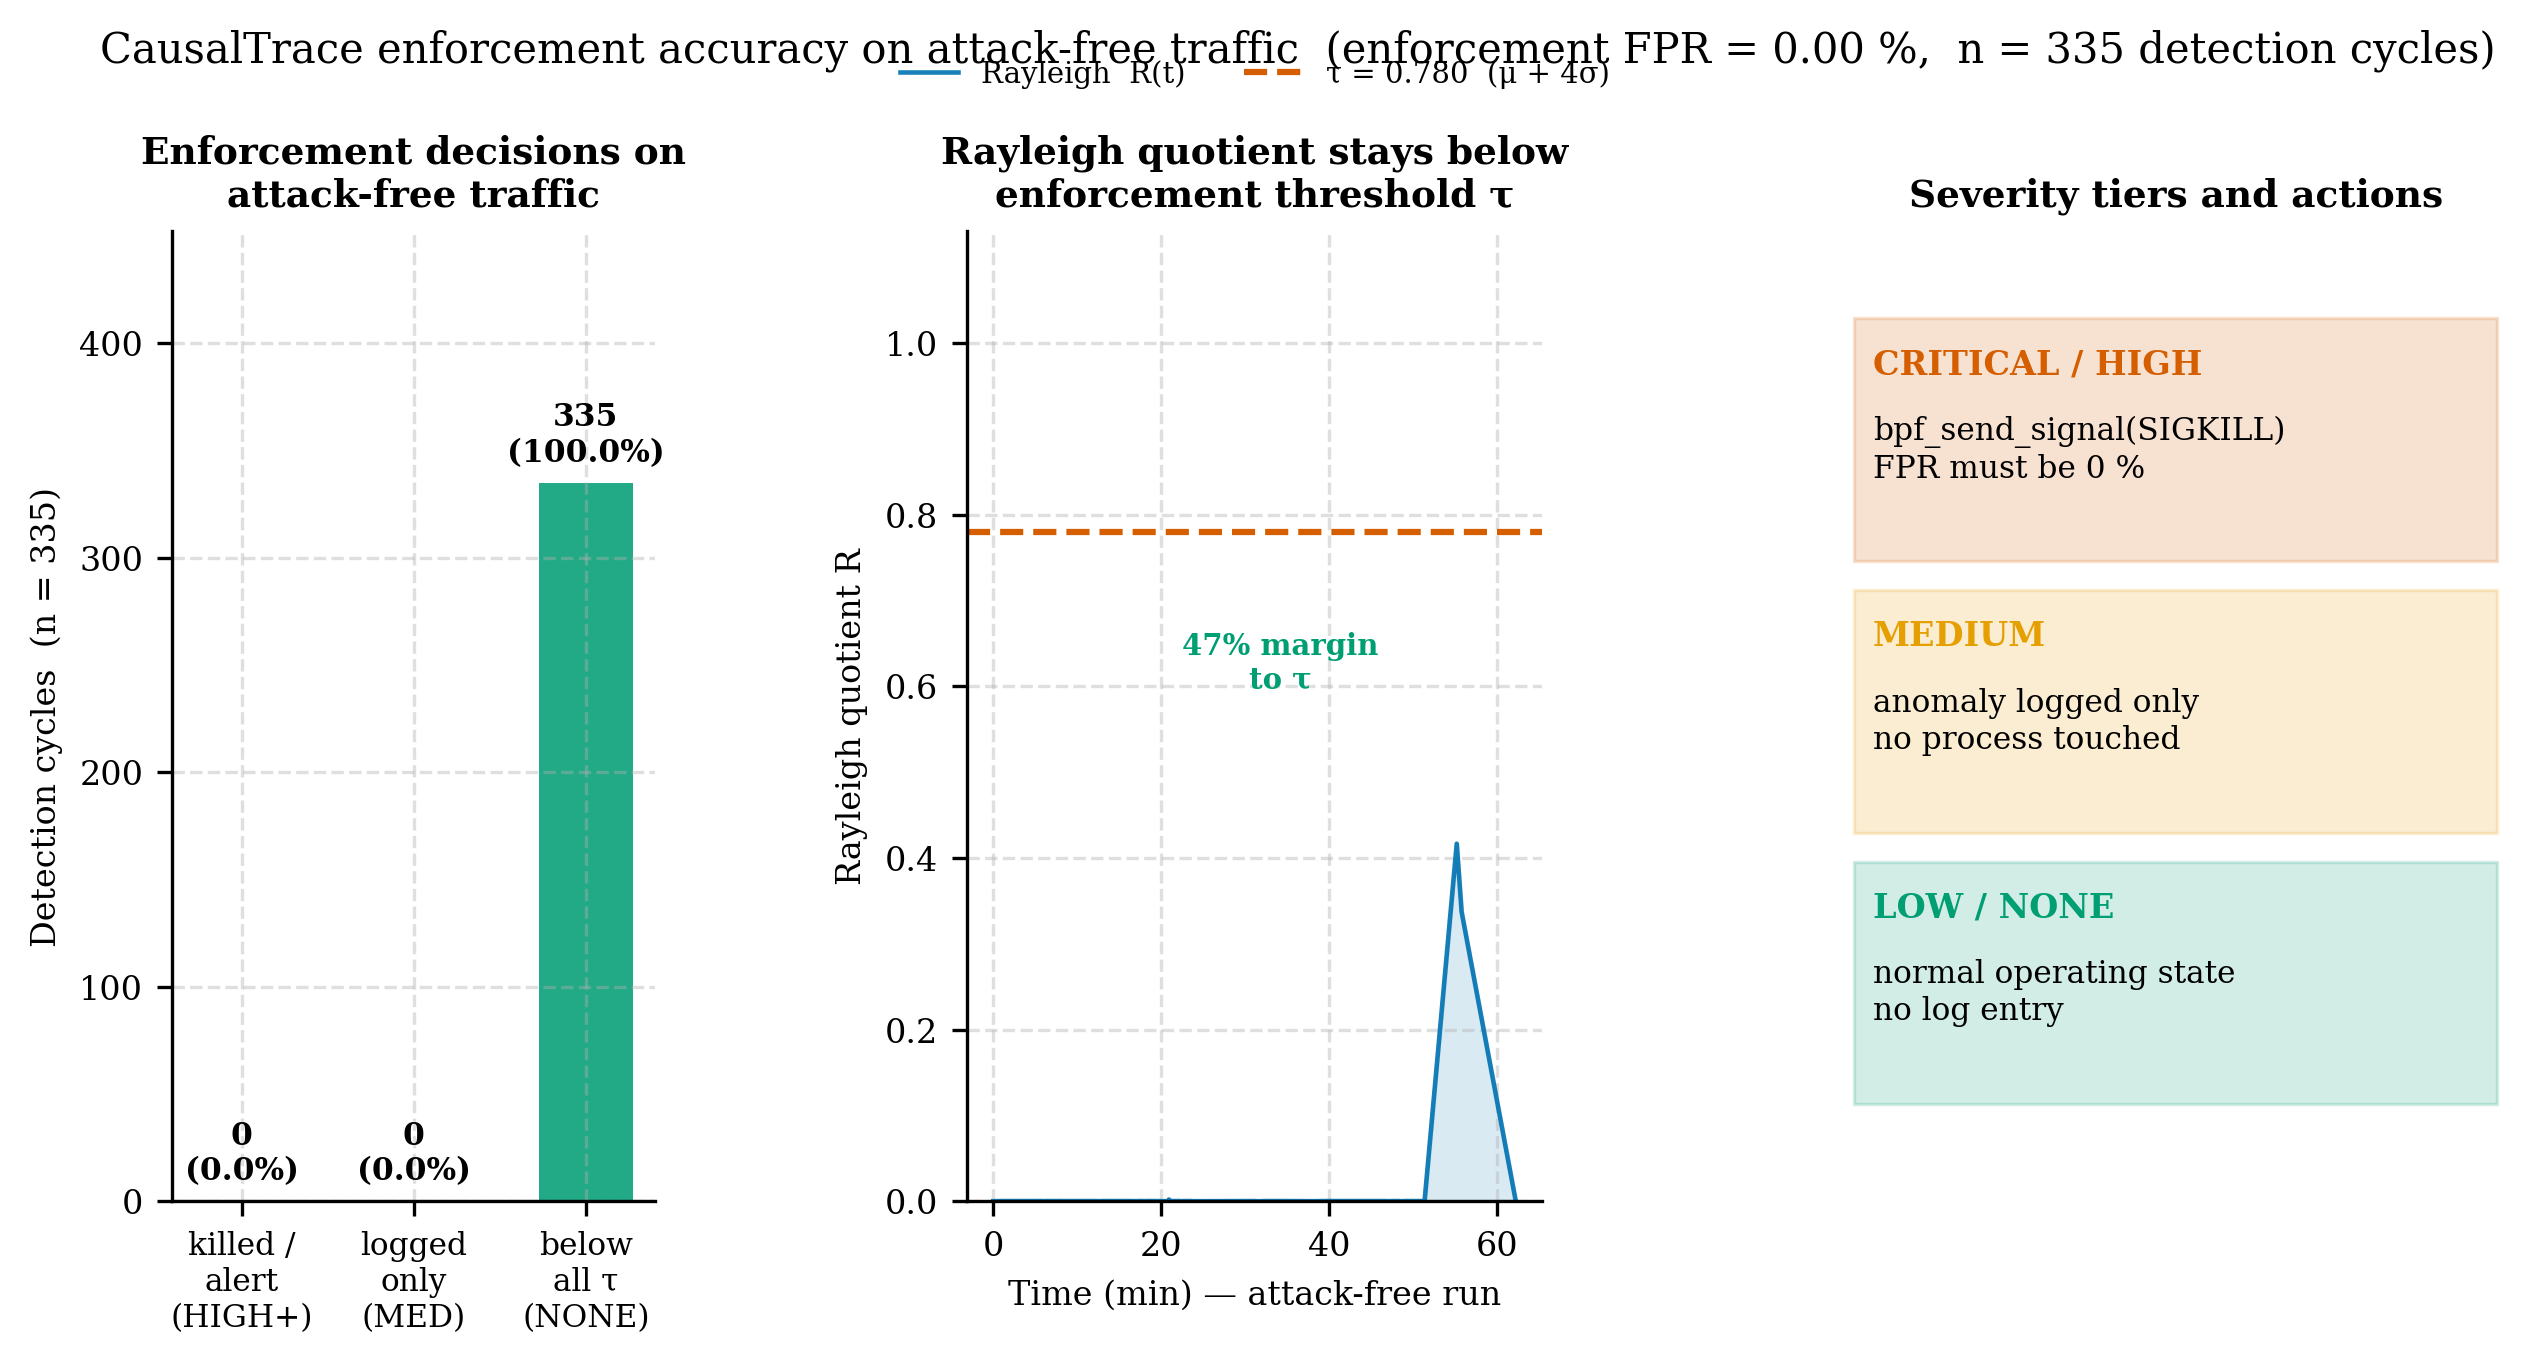
\includegraphics[width=0.9\linewidth]{figures/fig_fpr_normal.png}
  \caption[Steady-state false-positive rate]{Per-layer alert rate on
  attack-free steady-state traffic. CausalTrace holds $\leq 1$
  alert~/~hour on the workload surface; Falco stock is noisier because
  of its general-purpose ruleset.}
  \label{fig:fpr-normal}
\end{figure}

%─────────────────────────────────────────────────────────────────────────────
\section{Out-of-distribution evaluation (S11)}
\label{sec:ood}
%─────────────────────────────────────────────────────────────────────────────

S11 is held out of the calibration set: the payload is staged through
\texttt{memfd\_create(2)}, written into the anonymous file descriptor,
and executed via \texttt{execveat(AT\_FDCWD, "/proc/self/fd/N", \ldots)}.
Nothing touches the disk.

CausalTrace catches all five S11 injections through Theorem~\ref{thm:invariant}:
the \texttt{memfd\_create} syscall is in the top-24 set tracked by the
dispatcher, and the subsequent \texttt{execveat} with an
\texttt{/proc/self/fd/\_} path trips the strict-invariant case in
\texttt{handle\_execve}. Falco tuned catches three of five through a
generic \texttt{memfd\_create} rule; Tetragon catches none.

Table~\ref{tab:ood} reports the OOD breakdown. The asymmetry is the
thesis claim: a system calibrated on \emph{known normal} recalibrates to
\emph{novel attacks} because physical invariants do not require
enumeration.

\begin{table}[h]
\centering
\caption[S11 OOD detection]{Detection of the held-out S11 fileless OOD
scenario (5 injections per detector).}
\label{tab:ood}
\small
\begin{tabular}{lcc}
\toprule
Detector             & S11 detected & Rate \\
\midrule
CausalTrace          & 5 / 5 & 100\,\% \\
Falco (stock)        & 3 / 5 & 60\,\% \\
Falco (tuned)        & 3 / 5 & 60\,\% \\
Tetragon (stock)     & 0 / 5 & 0\,\% \\
Tetragon (tuned)     & 0 / 5 & 0\,\% \\
\bottomrule
\end{tabular}
\end{table}

%─────────────────────────────────────────────────────────────────────────────
\section{Tier attribution and runtime overhead}
\label{sec:tier-overhead}
%─────────────────────────────────────────────────────────────────────────────

Figure~\ref{fig:tier-breakdown} decomposes CausalTrace detections by the
tier that fired first. Tier-1 invariants cover the single-container
classes (S2, S2a, S3, S3a, S4, S5, S6, S11). The cross-container
classes (S7, S8, S9, S10) are confirmed by Tier-3 sheaf anomalies.

\begin{figure}[t]
  \centering
  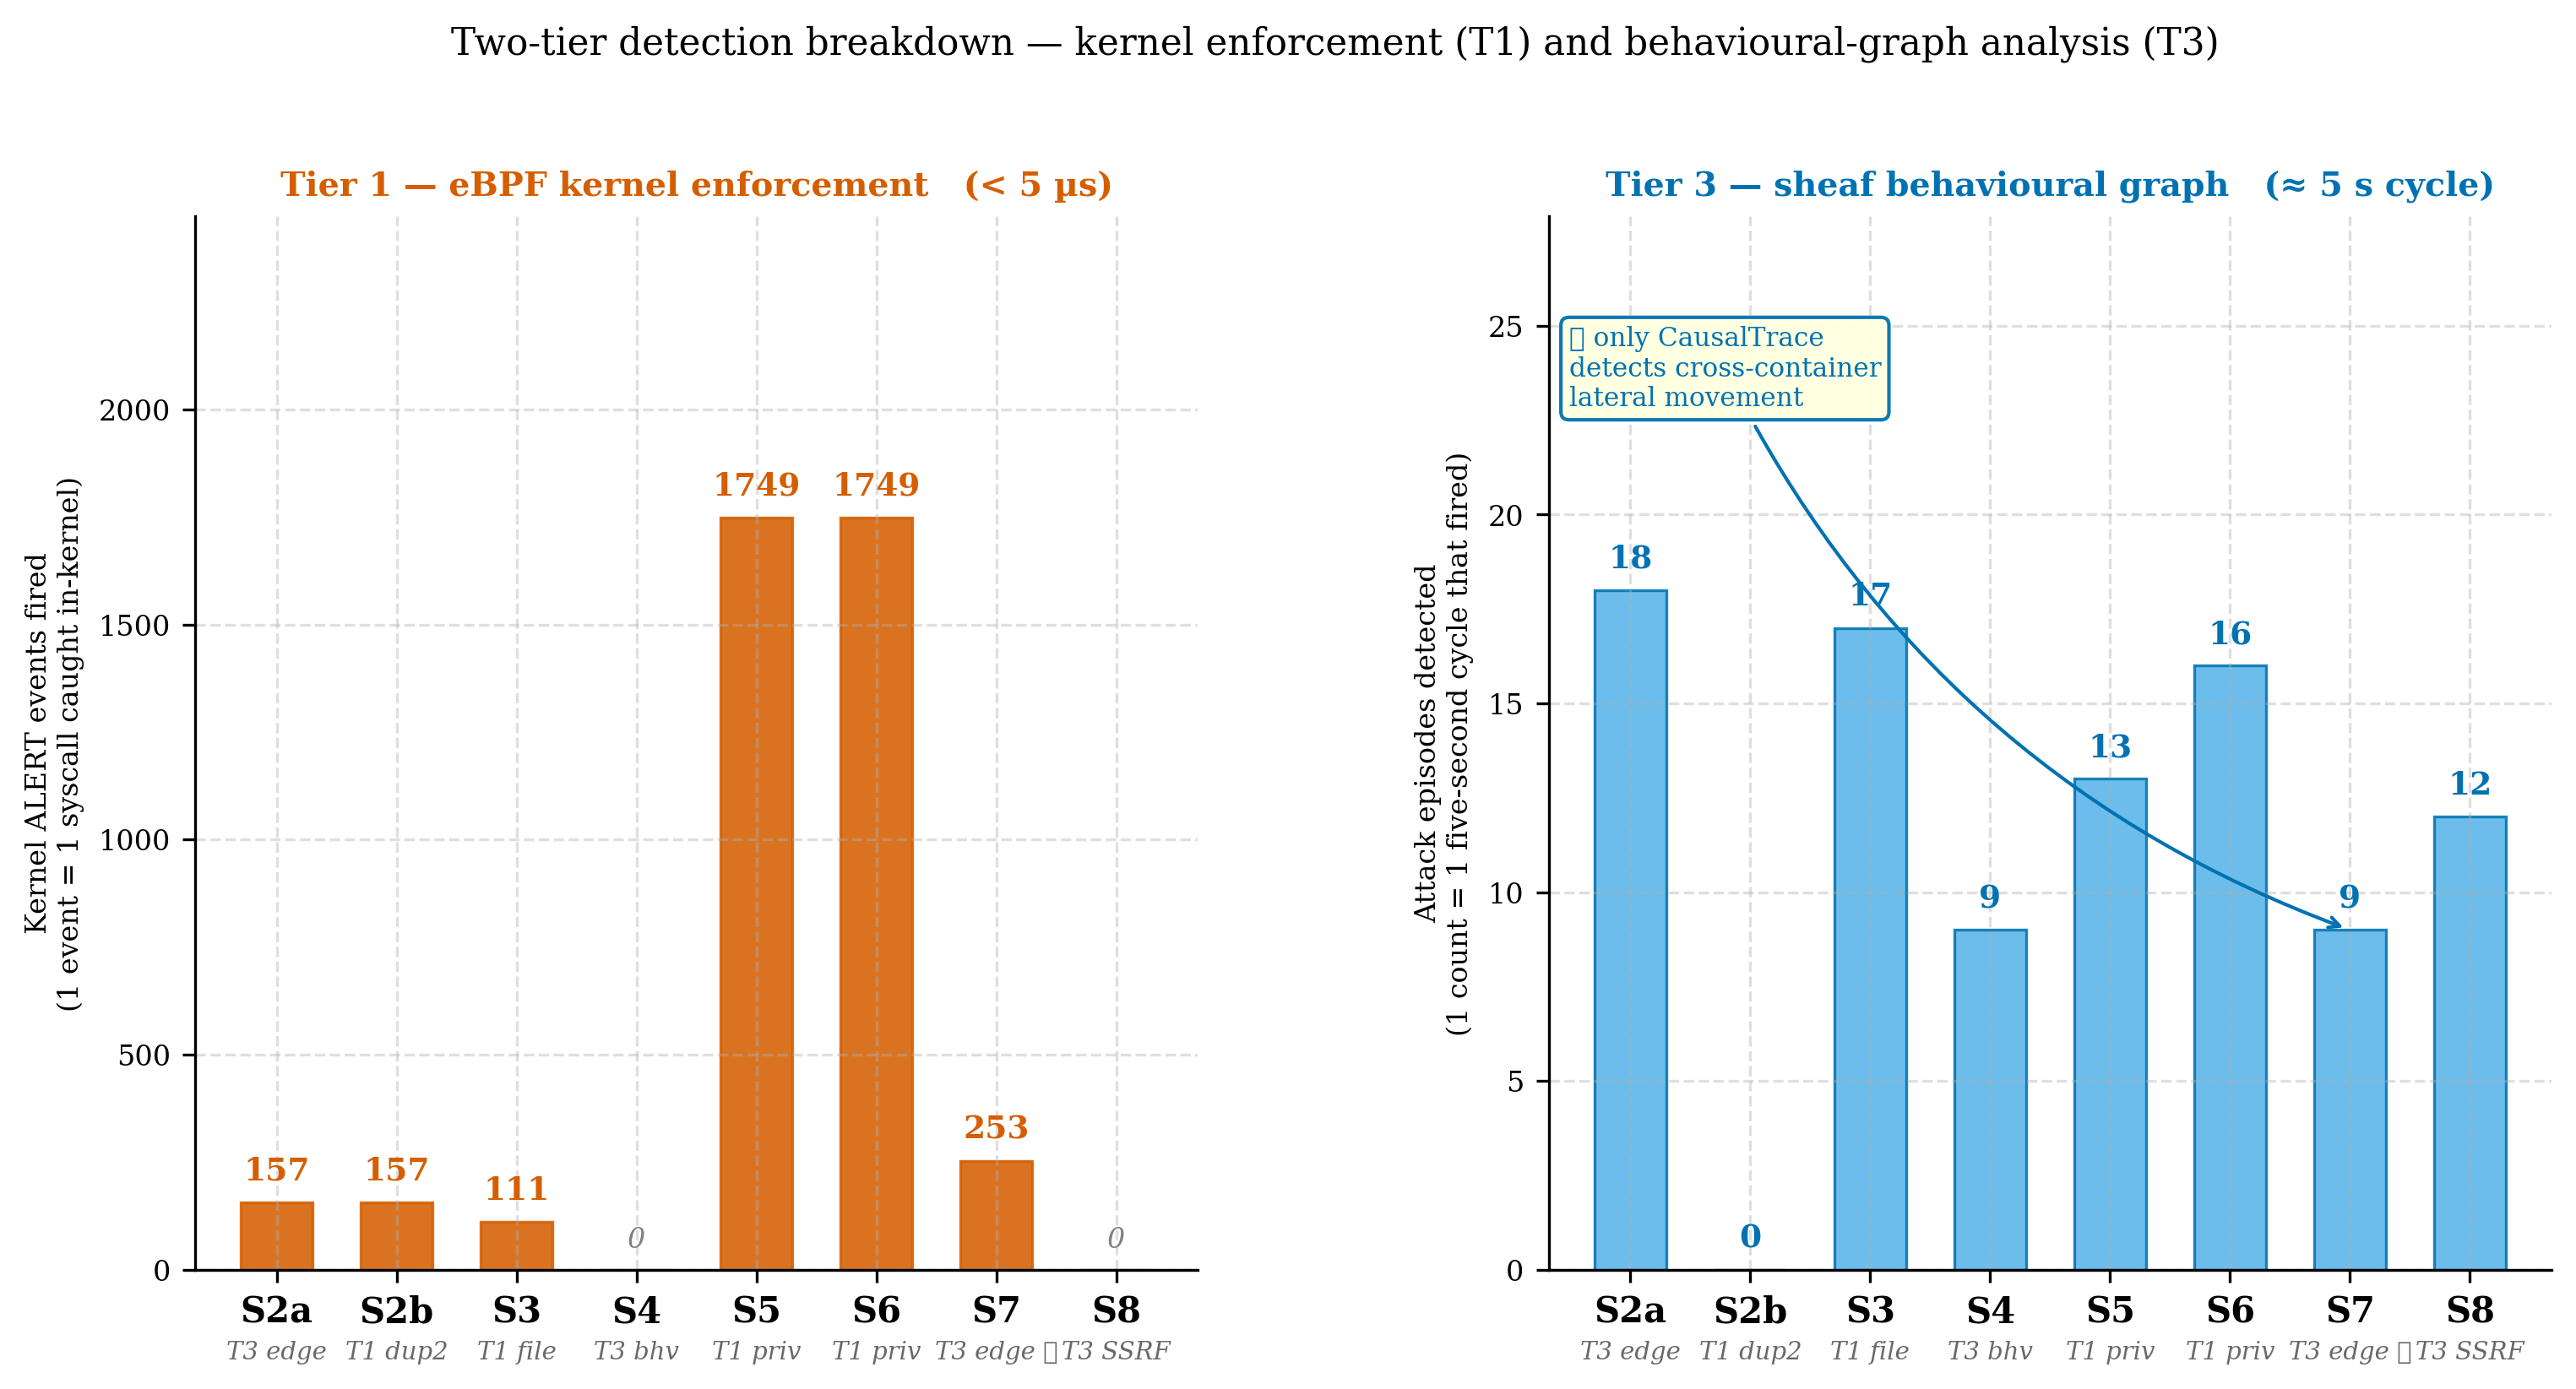
\includegraphics[width=\linewidth]{figures/fig_tier_breakdown.png}
  \caption[Tier breakdown per scenario]{Per-scenario detection
  attribution by tier. Tier-1 dominates the in-container classes;
  Tier-3 dominates the cross-container and chain classes. The two
  surfaces cover complementary subsets of the attack space.}
  \label{fig:tier-breakdown}
\end{figure}

\begin{figure}[t]
  \centering
  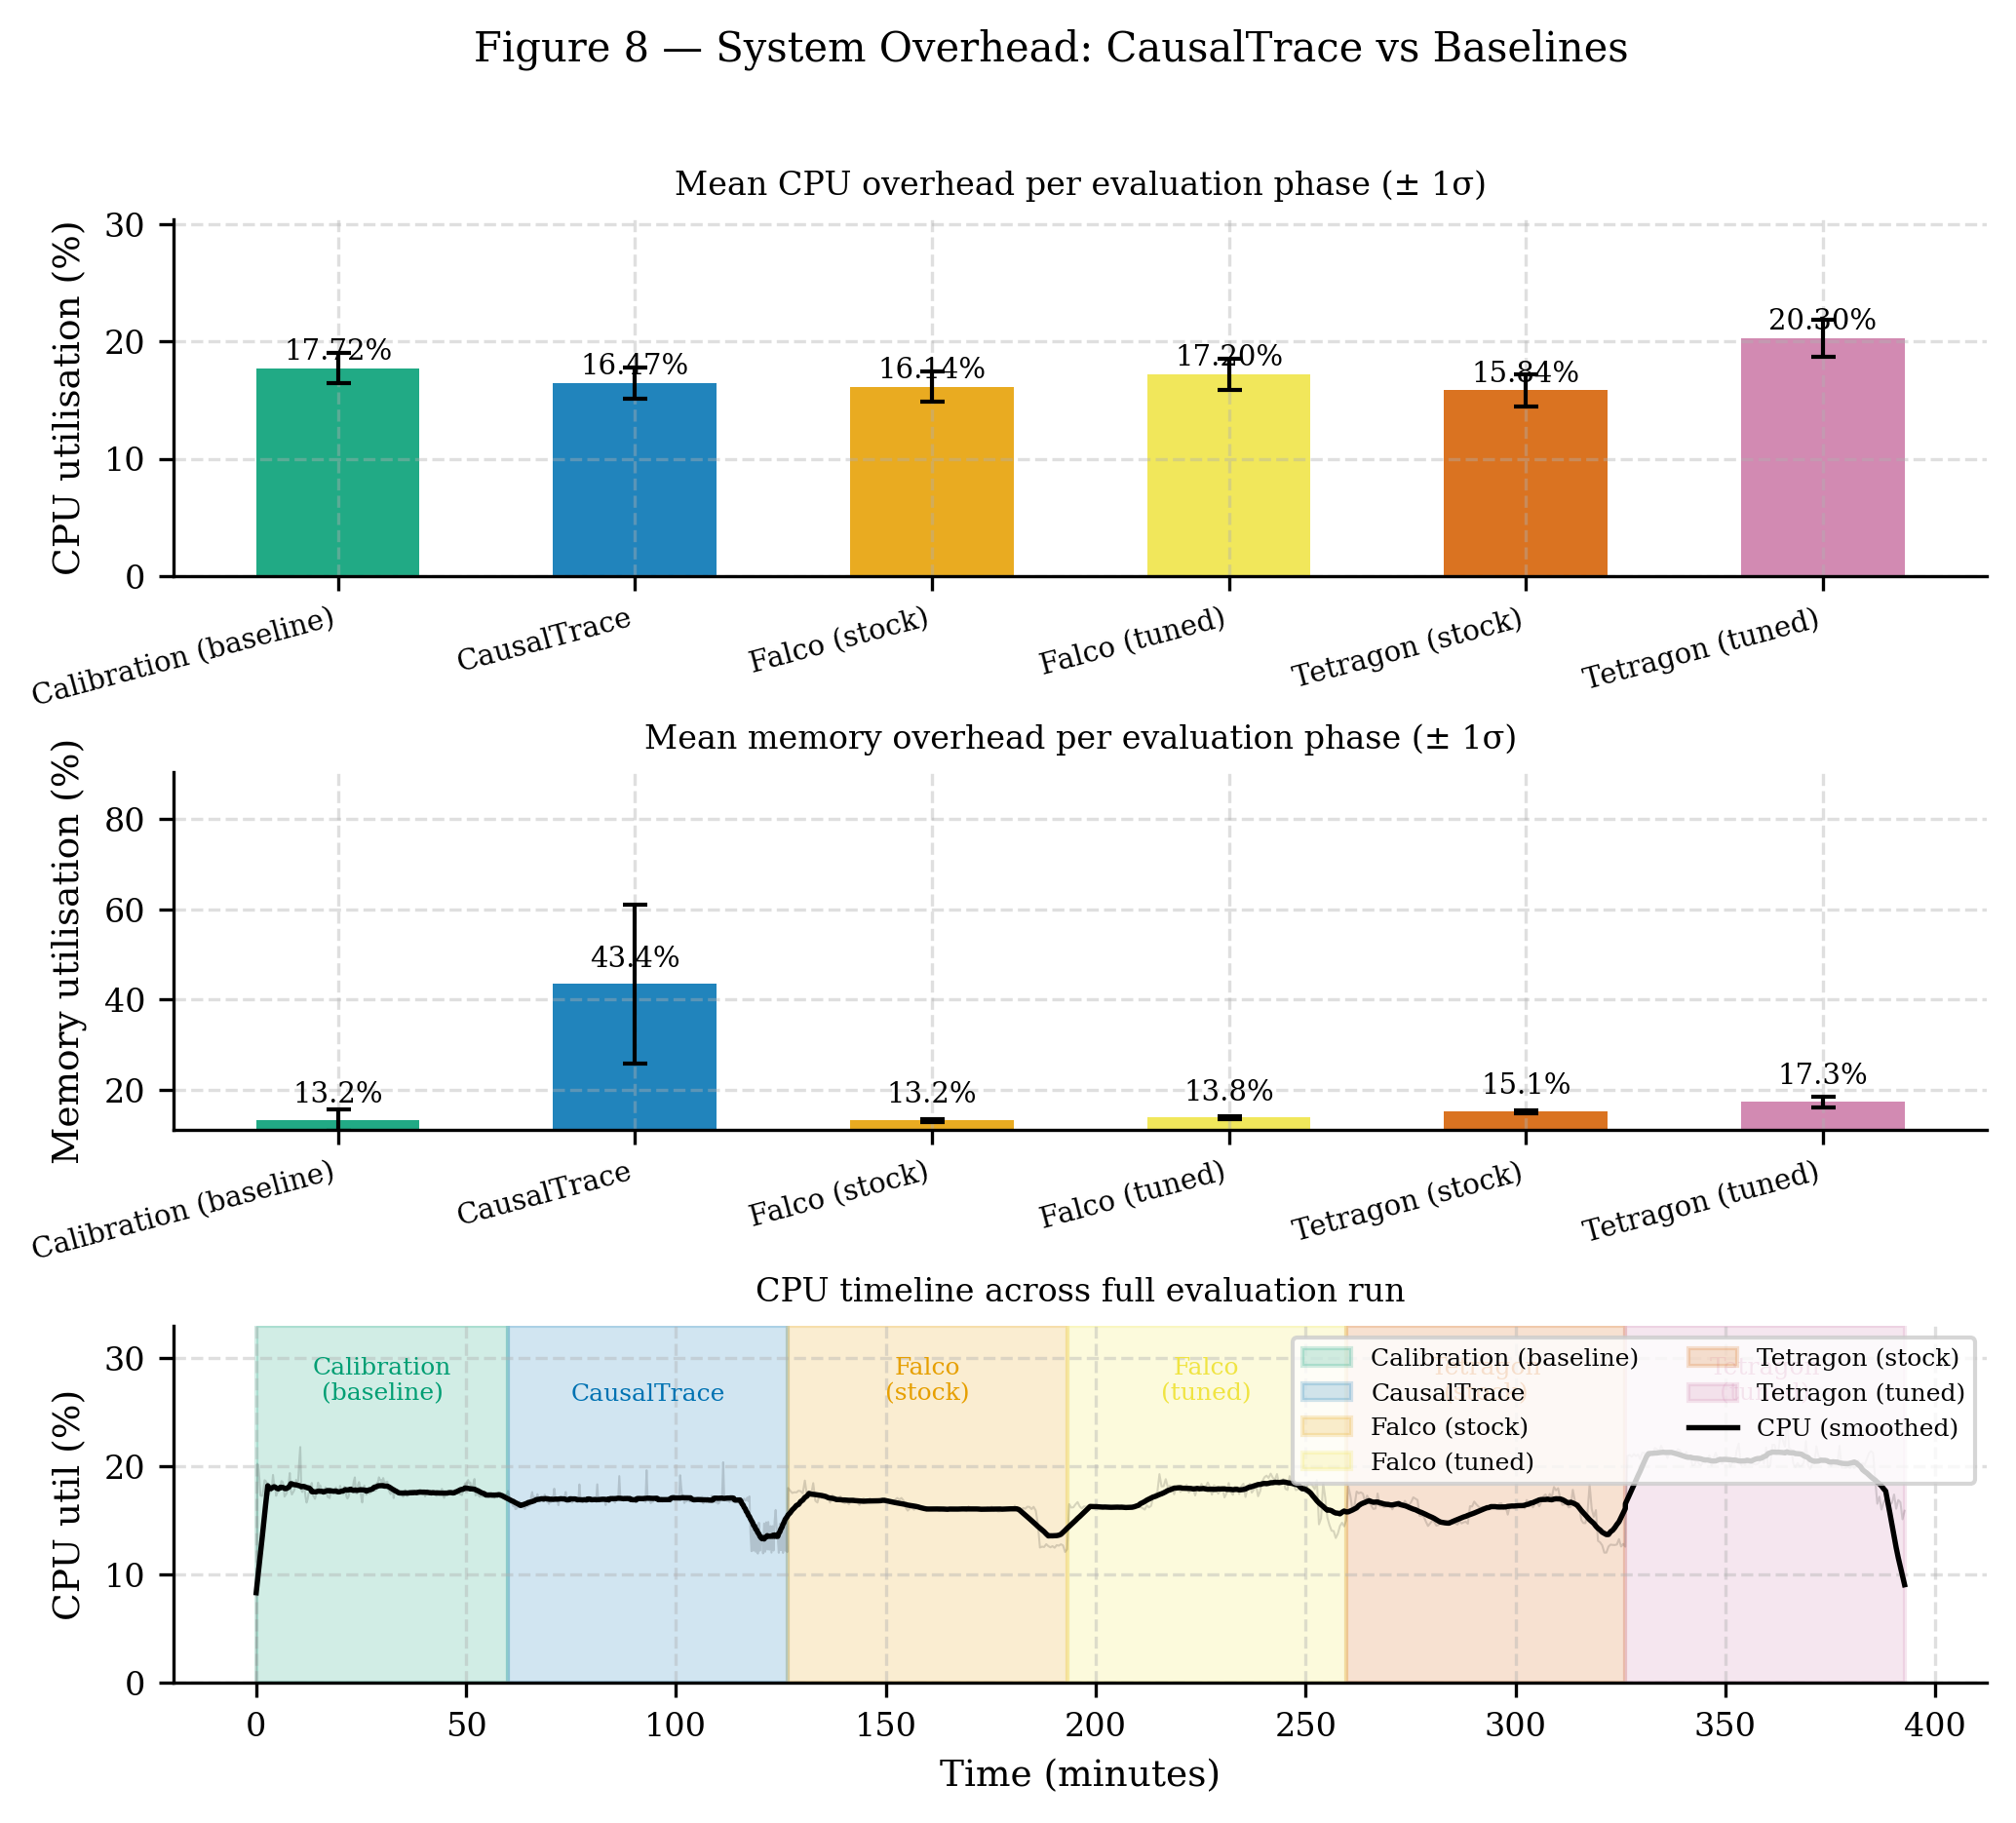
\includegraphics[width=\linewidth]{figures/fig_runtime_overhead.png}
  \caption[Runtime overhead]{Runtime overhead on a \texttt{wrk}-driven
  load against ct-nginx. CausalTrace's $\approx 1\,\%$ throughput impact
  is dominated by the \texttt{bpf\_probe\_read\_kernel} indirection
  forced by the verifier workaround of Chapter~\ref{Chapter5}.}
  \label{fig:runtime-overhead}
\end{figure}

%─────────────────────────────────────────────────────────────────────────────
\section{Threats to validity}
\label{sec:threats}
%─────────────────────────────────────────────────────────────────────────────

Four threats shape how these results should be read. Cross-kernel
generalisation is plausible but unverified: all results come from a
single evaluation host on Linux~6.17, and the verifier workarounds of
Chapter~\ref{Chapter5} are kernel-version-specific. Testbed realism is
bounded: the 22-container mesh reproduces a realistic service graph but
the workload generated by \texttt{wrk} and docker-exec is synthetic.
Baseline tuning introduces a pro-CausalTrace bias: we tuned Falco and
Tetragon for this attack set, which is also the set CausalTrace is
designed to catch, so stock numbers under-count what a production Falco
operator would write. Finally, the Wilson interval at $\hat{p}=1.00$
with $n=15$ per scenario has lower bound $\approx 0.80$, so a scenario
reporting 15/15 could plausibly be an 80\,\% detector; aggregate
intervals across the 155-injection set are much tighter.
